\section{Hypothesentests}
\subsection{PE-File Korrumpierung bei mehrstufiger Obfuskierung}
Das Experiment hat gezeigt, dass insgesamt 23,4\% der vorhandenen Samples korrumpiert waren. Von den mehrstufigen Obfuskationen waren 0.7\% korrumpiert. Der Anteil an Korrumpierung unter den mehrstufigen Obfuskationen lag bei 1,4\%.  Allerdings zeigt sich in Tabelle \ref{tab:corrupted_files}, dass die meisten Korruptionen bei Windows Defender aufgetreten sind und unter MDE fast keine. Insgesamt sind die mehrstufigen Korruptionen deutlich seltener gewesen als die einstufigen korrupten Files. Dies kann ein Ergebnis des genetischen Algorithmus sein, der die Lösungen Teil für Teil konstruiert und so viele fehlerhafte einstufige Teile hat, bevor er die erfolgreichen mit anderen Kandidaten rekombiniert. 
In keinem der Fälle wurde das Niveau von 25\% überschritten, was dafür spricht, dass ein Großteil der dargebotenen Files eine sehr solide Rate von Ausführbarkeit beweist und der Algorithmus nicht langwierig in unausführbaren Stacks herumsucht. Gegenüberstellung der Korrumpierungsanteile von allen Dateien gegen die mehrstufigen Dateien findet sich in Abbildung \ref{fig:corrupt_vs_multi}.

\begin{figure}[h]
    \centering
    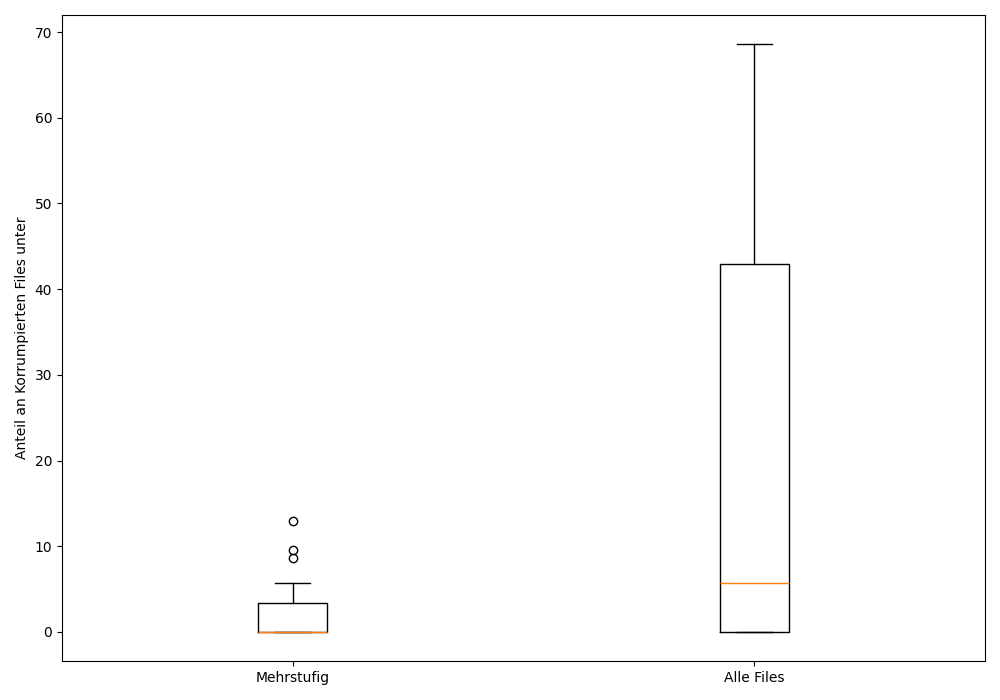
\includegraphics[width=0.85\textwidth]{gfx/Hypothesendiagramme/corruption_vs_multi_corruption.png}
    \caption{Anteil der Korrumpierten Dateien}
    \label{fig:corrupt_vs_multi}
\end{figure}

\subsubsection{Testauswahl}
Aufgrund der geringen Stichprobe von \textit{N = 18} wurde sich gegen einen Z Test und für einen Binomialtest anhand der Anteile von Korruption entschieden, der wie in Codebeispiel \ref{Code:Corruption_test} durchgeführt wurde.

\begin{listing}
    \begin{minted}{Python}
corrupted_multiparts_over_number_multiparts= 
    [0.0, 0.0, 0.0, 0.0,  0.0, 0.0,
    0.04545, 0.06667, 0.0, 0.0, 0.0, 0.03,
    0.0,  0.05, 0.0, 0.0, 0.0, 0.0]
print(np.mean(corrupted_multiparts_over_number_multiparts))
print(percentage_corrupt_of_multiparts)
n = len(percentage_corrupt_of_multiparts)
k = sum(1 for p in percentage_corrupt_of_multiparts if p >0.25)
p_value_binom= binomtest(k,n, p =0.25, alternative='greater')
print(p_value_binom)
    \end{minted}
    \label{Code:Corruption_test}
    \caption{Hypothesentest Korrumpierte mehrstufige}
\end{listing}

\subsubsection{Ergebnis}
Der Test hat einen mittleren Korrumpierungsanteil von 1,06\% ergeben. Der P-Test (\textbf{p = 1.0} hat die Nullhypothese von einem Anteil von kleiner-gleich 25\% beibehalten und die Hypothese somit wiederlegt.

\subsubsection{Weitere Überprüfung}
Der gleiche Test wurde mit dem Anteil aller korrumpierten Files an allen erstellten Files wiederholt und ergab dabei einen Mittelwert von 23,4\% und einen p-Wert von 0.019. Hierbei lässt sich also tatsächlich eine Tendenz von mehr als 25\% korrumpierter Dateien vermuten.

% subsection{Geringe Shellcode Korrumpierung}
% Todo bei neuem Experiment
% 
%\textbf{Eventuelle Streichung bei keiner Verbesserung des Ergebnisses}

\subsection{Red-Teaming Kriterien Erfüllung}
Aus dem Experiment hat sich - abgesehen von den architektonischen Details - gezeigt, dass die zwei wesentlichen Anforderungen für den praktischen Einsatz mit den gestellten Konfigurationen erfüllt werden können.
So hat sich nicht nur gezeigt, dass die Laufzeit aller Experimente (Tabelle \ref{tab:runtime}) unterhalb der Zeit lag, die maximal verwendet werden darf, sondern auch gezeigt, dass in jedem Experiment mindestens eine erfolgreiche Evasion Lösung erstellt werden konnte\footnote{Eine Wiederholung des Algorithmus war nötig, aber die zusätzliche Zeit wurde mit einberechnet}, die von einem AV Scanner nicht erkannt wurde. Auch könnte man die Laufzeit des Algorithmus noch weiter optimieren, indem der Algorithmus sofort beim finden einer einzelnen Lösung terminiert und somit potentiell weitere Zeit erspart. Für die Fragestellung war dies jedoch nicht zielführend, weswegen dieses Feature hier nicht implementiert worden ist.

\subsubsection{Testauswahl}
\subsubsection{Testergebnis}
\subsubsection{Weitere Betrachtung}
Zeit pro Lösung und Optimierungsmöglichkeiten


\subsection{Einfluss der Länge von Obfuskatorkaskaden}

 \subsubsection{Testauswahl}
 Da es für diesen Test zwei unabhängige Variablen (AV Scanner und Malware Typ) und nur eine abhängige Variable (Anzahl der Obfuskationsschritten von Erfolgreichen Kandidaten) gibt, wird hier eine zweifaktorielle ANOVA durchgeführt.\footnote{Code von ChatGPT erstellt nach Beschreibung der vorhandenen Daten}

\begin{listing}
    \begin{minted}{Python}
import statsmodels.api as sm
import pandas as pd
from statsmodels.formula.api import ols

data ={
    'Malware_Type': ['Benign']*24 + ['Calc']*24 + ['Shell']*15,
    'AV_Scanner': ['MDE']*10 + ['WD']*14 + 
        ['MDE'] *15 + ['WD'] *9 + 
        ['MDE']*11 + ['WD']*4,
    'Steps':  [1]*8+[2]*2+[1]*9+[2]*4+[4] + 
        [1]*5 + [2]*10 + [1]*5 + [2]*4+ 
        [2]*9 + [3]*2 + [2]*4
} 

df = pd.DataFrame(data)
model = ols('Steps ~ C(Malware_Type) * C(AV_Scanner)', data=df).fit()
anova_table = sm.stats.anova_lm(model, typ=2)

print(anova_table)
    \end{minted}
\end{listing}

 \subsubsection{Testergebnis}
 In Tablle \ref{ANOVA} sieht man die Ergebnisse der multifaktoriellen ANOVA. Es stellt sich heraus, dass der Malware Typ als einziges einen signfikanten Unterschied in den nötigen Schritten bewirkt und weder der AV-Scanner noch das AV-Scanner - Malware Typ Paar signifikant zur Varianzaufklärung beitragen.
\begin{table}[hp]
\begin{tabular}{@{}lllll@{}}
\toprule
                           & sum\_sq   & df   & F        & PR(\textgreater{}F) \\ \midrule
Malware Typ                & 5.113966  & 2.0  & 7.967892 & \textit{0.000888}            \\
AV Scanner                 & 0.000077  & 1.0  & 0.000241 & 0.987679            \\
Malware Typ und AV Scanner & 0.899670  & 2.0  & 1.401745 & 0.254523            \\
Residual                   & 18.291919 & 57.0 & NaN      & NaN                 \\ \bottomrule
\end{tabular}
\label{ANOVA}
\caption{ANOVA Ergebnis Obfuskationsschritte}
\end{table} 
\begin{figure}[h]
    \centering
    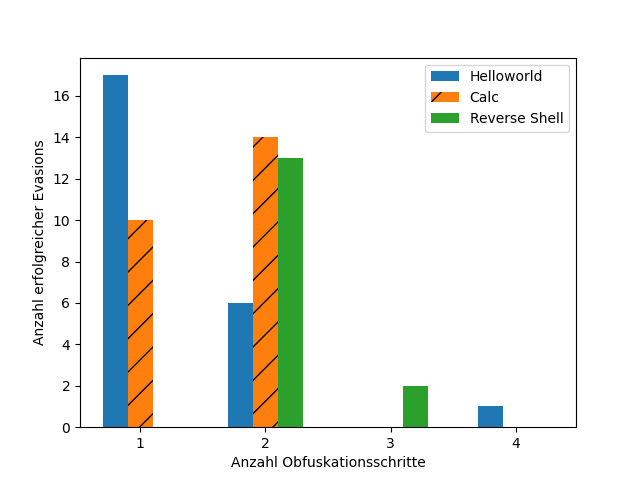
\includegraphics[width=0.85\textwidth]{gfx/Hypothesendiagramme/combined_obfuscation_steps.png}
    \caption{Anzahl der Obfuskationschritte bei erfolgreichen Kandidaten in Abhängigkeit vom Malwaretyp}
    \label{fig:steps_per_Solve}
\end{figure}

\subsubsection{weitere Betrachtung}
Wie bereit ins \ref{fig:steps_per_Solve} absehbar, zeichnet sich ein Trend ab, was die nötigen Obfuskationsschritte pro Malwaretyp angeht. So scheint es, dass Shell Access Malware längerstufige Obfuskationsschritte benötigt, als die anderen beiden getesteten Files. Für die Benign-Testcases hat sich weiterhin gezeigt, dass am häufigsten eine kurze Lösung zum Erfolg führte, aber auch eine (unnötig) lange Lösung mit 4 Schritten dem Scanner entgehen konnte. Ein möglicher Schluss lautet, dass die Freiheitsgrade, die zur Evasion zur Verfügung stehen, geringer werden, je interaktiver Malware ist. Dies würde zumindest erklären, warum bei dem Benigntestcase auch Lösungen mit 4 Schritten erfolgreich waren.

\subsection{Zusammenfassung}
\begin{table}[h]
    \centering
    \begin{tabular}{|l|l|l|}
        \hline
        \textbf{Hypothese} & \textbf{Ergebnis} & \textbf{Indizien} \\ \hline
        Hypothese 1: PE Korrumpierung steigt mit dem Stapeln von Obfuskationen & Widerlegt& \ref{fig:corrupt_vs_multi} \\ \hline
        Hypothese 2: Red Teaming Kriterien erfüllbar & Bestätigt & Zusammenfassung der Indizien \\ \hline
        Hypothese 3: Zusammenhang von Malware Typ mit nötiger Obfuskation & Bestätigt & ANOVA Tab. \ref{ANOVA} \\ \hline
    \end{tabular}
    \caption{Übersicht über die Hypothesenprüfung des Papers}
    \label{tab:hypothesenpruefung}
\end{table}